% !TeX root = ../main.tex
\chapter{Konzipierung der Lösung}
\label{cha:konzept}
% WARUM und WAS: Systemkonzept, Architektur, Entwurfsentscheidungen — jeweils
% mit Bezug auf die Anforderungs-IDs. Das WIE gehört in die Implementierung.

\section{Konzept und System}
\label{sec:konzept}
% Beispieltext zum Sequenzdiagramm — Aufbau übernehmen, Inhalt ersetzen.

Das zeitliche Zusammenspiel der Komponenten beim Laden von Daten zeigt
\autoref{fig:sequenz-beispiel}. Die Web-App sendet die Anfrage asynchron an den
Webserver und bleibt währenddessen bedienbar; eine Ladeanimation zeigt den
laufenden Vorgang an. Der Webserver fragt die Datenbank dagegen synchron ab und
ist bis zum Eintreffen der Ergebniszeilen blockiert. Anschließend wandelt er die
Zeilen in das JSON-Format um und beantwortet die ursprüngliche Anfrage. Den
Ablauf innerhalb einer einzelnen Komponente zeigt der Programmablaufplan in
\autoref{fig:pap-beispiel} im Anhang (\autoref{sec:anhang-pap}).

\begin{figure}[H]
    \centering
    % Quelle: assets/diagrams/sequenzdiagramm.md (Mermaid)
    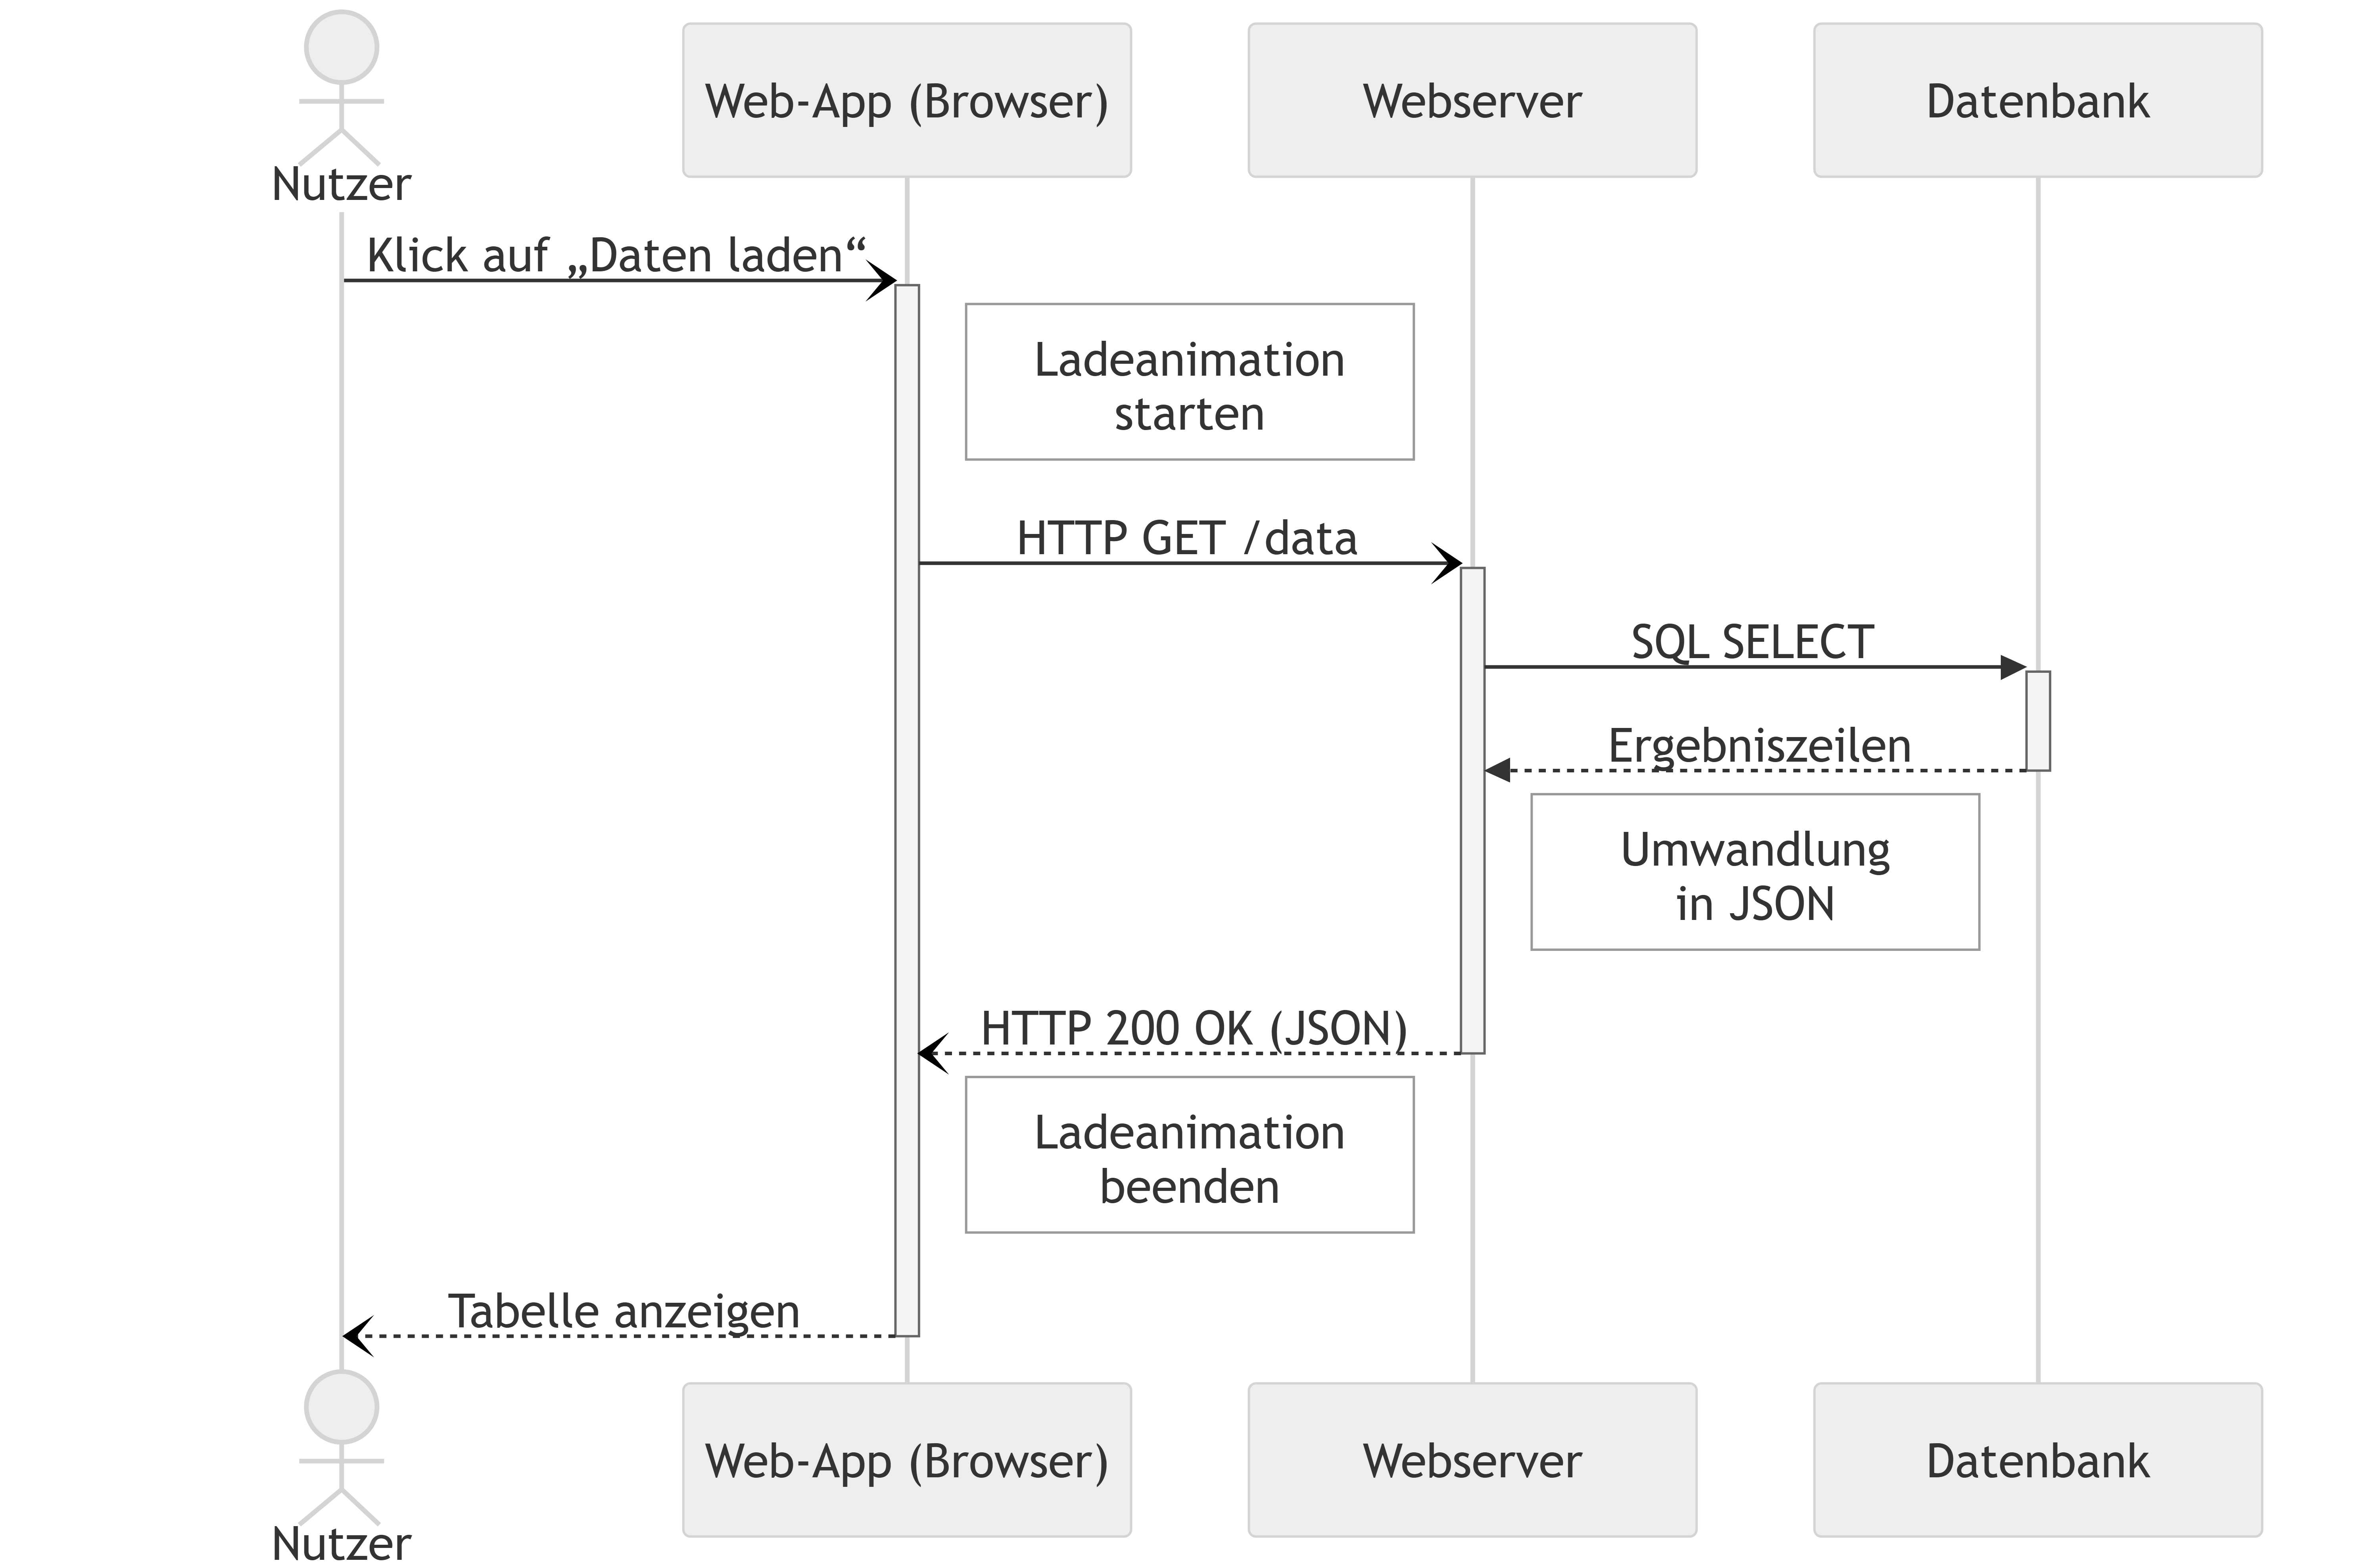
\includegraphics[width=0.9\textwidth]{assets/diagrams/sequenzdiagramm.png}
    \caption{Sequenzdiagramm einer Datenabfrage mit asynchroner HTTP-Anfrage und
        synchronem Datenbankzugriff (Beispiel)}
    \label{fig:sequenz-beispiel}
\end{figure}

% Die beiden folgenden Abschnitte stehen am Ende dieses Kapitels und sind bei
% vielen Prüfern Pflicht.
\section{Verwendete Hard- und Software}
\label{sec:hard-software}
% Komponenten, die im Betrieb der Lösung laufen — mit Versionsangaben
% (Tabelle). Bei Abhängigkeiten mit Versionsbereich die tatsächlich aufgelöste
% Version nennen.

\section{Verwendete Entwicklungs- und Hilfsmittel}
\label{sec:hilfsmittel}
% Entwicklungsumgebung inkl. Erweiterungen, Build- und Diagrammwerkzeuge —
% und SÄMTLICHE KI-Werkzeuge mit Modell und Einsatzzweck. Die Erklärung zur
% Selbständigkeit verweist hierher. Beispieltext unten an die eigene Nutzung
% anpassen; nichts angeben, was nicht tatsächlich genutzt wurde. Die
% Versionen stehen in VS Code unter Erweiterungen bzw. Hilfe > Info.

Als Entwicklungsumgebung diente Visual Studio Code (Version~\dots) mit den
folgenden Erweiterungen:
\begin{itemize}[itemsep=0pt, parsep=0pt, topsep=4pt]
    \item \textit{LaTeX Workshop} (Version~\dots) -- Übersetzung der Ausarbeitung
        mit \texttt{latexmk} und PDF-Vorschau mit SyncTeX,
    \item \textit{Claude Code} (Version~\dots) und das integrierte \textit{GitHub
        Copilot} -- KI-Assistenten im Editor, siehe die Aufstellung der
        KI-Werkzeuge unten,
    \item \textit{Explorer Exclude Manager} (Version~\dots) -- Ausblenden von
        Build- und Hilfsdateien im Dateiexplorer.
\end{itemize}

Als weiteres Hilfsmittel kam \ac{ki} zum Einsatz. Die folgende Aufstellung nennt
die verwendeten Werkzeuge, die dabei genutzten Modelle und den jeweiligen
Einsatzzweck:
\begin{itemize}[itemsep=0pt, parsep=0pt, topsep=4pt]
    \item \textbf{Werkzeug A} (Hersteller, Version) -- Modelle: \dots; Einsatz: \dots
    \item \textbf{Werkzeug B} (Hersteller, Version) -- Modelle: \dots; Einsatz: \dots
\end{itemize}

Sämtliche mit KI-Unterstützung entstandenen Ergebnisse wurden vor der Übernahme
geprüft und überarbeitet; die fachliche Verantwortung für alle Teile der Arbeit
liegt beim Verfasser.
